\section{Ausführung in Matlab}

\subsection{LLS-Realisierung in MATLAB}
P\textsubscript{1} bis P\textsubscript{5} sind die Referenzpunkte mit den Koordinaten (X\textsubscript{1}, Y\textsubscript{1}, Z\textsubscript{1}) bis (X\textsubscript{5}, Y\textsubscript{5}, Z\textsubscript{5}) und R\textsubscript{1} bis R\textsubscript{5} die gemessene Distanzen. Folgende Referenzpunkte und Distanzmessungen sind gegeben (Einheit: Meter):
\begin{flushleft}
	P\textsubscript{1} = (10, 0, 0), R\textsubscript{1} = 10.02;\\
	P\textsubscript{2} = (0, 10, 0), R\textsubscript{2} = 10.05;\\
	P\textsubscript{3} = (0, 0, 10), R\textsubscript{3} = 9.98;\\
	P\textsubscript{4} = (-10, 0, 0), R\textsubscript{4} = 10.07;\\
	P\textsubscript{5} = (0, -10, 0), R\textsubscript{5} = 9.99;
\end{flushleft}

In MATLAB werden zuerst obige Koordinaten und Distanzen eingegeben und das lineare Gleichungssystem (3) erstellt. Danach wird die gesuchte Position P\textsubscript{lat} mit den Formeln (4) und (5)  bestimmt. Das errechnetes Ergebnis lautet  X = 0.0168, Y = -0.0301 und Z = 0.0568. Die Wahre Position ist P\textsubscript{wahr} = (0.00, 0.00, 0.00). Das Ergebnis ist sehr zufriedenstellend, obwohl es kleine Abweichungen bei praktischen Distanzmessungen gibt. Vorher wurde bereits angesprochen, dass das Ergebnis schlecht berechnet werden kann wenn eine Distanzmessung stark von der wahren Distanz abweicht. Die Distanz von R\textsubscript{1} = 15.02 ist aufgrund von NLOS-Messung, so ist die gesuchte Position P\textsubscript{lat} = (-4.16, -0.03, 2.14) (vgl. Abb.3). Das Ergebnis weicht stark von P\textsubscript{wahr} = (0.00, 0.00, 0.00) ab. Um solche fehlerbehaftete Distanzmessungen zu filtern, ist Least Median Square sinnvoll.
\begin{figure}[H]
	\centering
	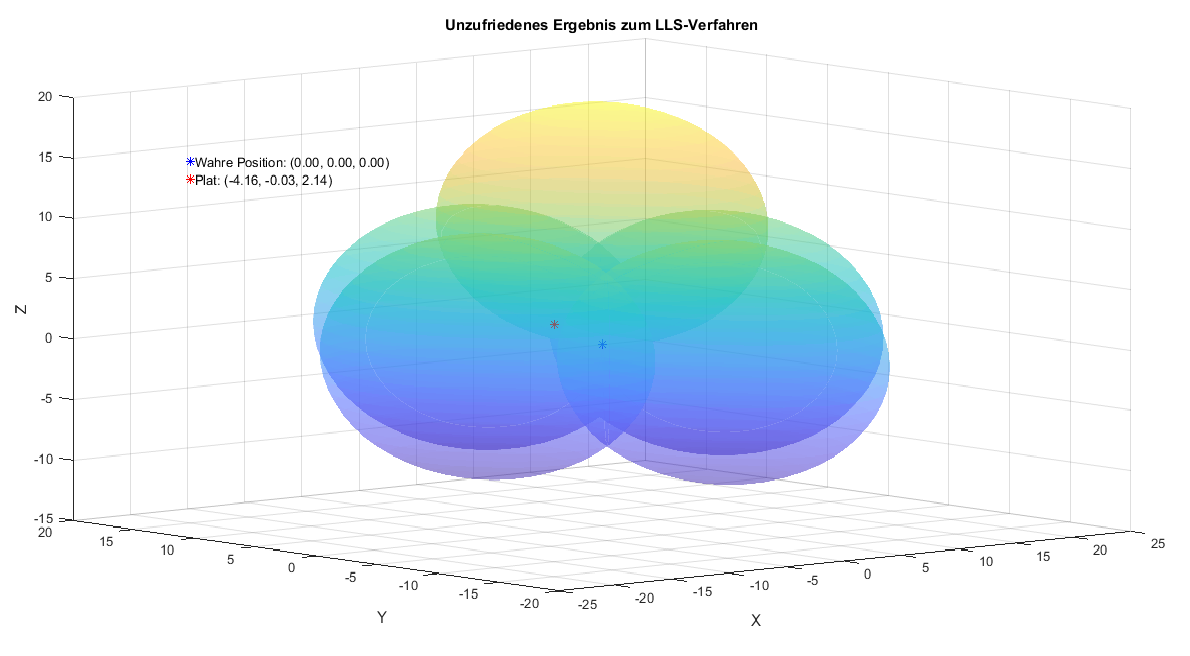
\includegraphics[scale=0.32]{img/Unzufriedenes_Ergebnis_zum_LLS-Verfahren.png}\\
	\caption{Unzufriedenes Ergebnis zum LLS-Verfahren }
\end{figure}

\subsection{LMS-Realisierung in MATLAB }
Mit den Formeln (6) und (7) kann die gesucht Position gefunden werden, die geringsten Medianwert hat. Damit können die fehlerbehaftete Distanzmessungen wegen NLOS-Messungen gefiltert werden. Jetzt ist ein Beispiel mit 6 Referenzpunkte gegeben. Alle Daten sind wie folgt dargestellt (Einheit: Meter): 
\begin{flushleft}
	P\textsubscript{1} = (10.00, 0.01, -0.01), R\textsubscript{1} = 10.20;\\
	P\textsubscript{2} = (0.02, 9.98, 0.01), R\textsubscript{2} = 9.88;\\
	P\textsubscript{3} = (0.01, 0.02, 9.56), R\textsubscript{3} = 9.54;\\
	P\textsubscript{4} = (-9.97, 0.02, 0.01), R\textsubscript{4} = 9.96;\\
	P\textsubscript{5} = (0.01, -10.01, 0.02 ), R\textsubscript{5} = 10.01;\\
	P\textsubscript{6} = (0.01, 0.03, -10.01), R\textsubscript{6} = 12.10;
\end{flushleft}
Es ist offensichtlich, dass die Distanzmessung R\textsubscript{6} zum Referenzpunkt P\textsubscript{6} durch NLOS-Messung von der wahren Distanz stark abgewichen ist und andere Distanzmessungen sehr gut sind. Hier ist die Wahre Position wieder P\textsubscript{wahr} = (0.00, 0.00, 0.00). 

In MATLAB werden zunächst die $(^6_4) = 15$ mögliche Kombinationen (\textit{Subsets}) verteilt, die von (P\textsubscript{1}, P\textsubscript{2}, P\textsubscript{3}, P\textsubscript{4}) bis (P\textsubscript{3}, P\textsubscript{4}, P\textsubscript{5}, P\textsubscript{6}) sind. Anschließend Position P\textsubscript{lat(k)} für jede Kombination mittels LLS-Verfahren ermittelt wird. Die gesuchte Postionen P\textsubscript{lat(1)} bis P\textsubscript{lat(15)} werden in MATLAB wie folgt ermittelt (Einheit: Meter):
\begin{flushleft}
P\textsubscript{lat(1)}: (-0.1059, 0.1959, 0.1202);\\
P\textsubscript{lat(2)}: (-0.2522, 0.0498, -0.0323);\\
P\textsubscript{lat(3)}: (0.9208,  1.2216, 1.1910);\\
P\textsubscript{lat(4)}: (-0.0086, 0.0984, 97.3134);\\
P\textsubscript{lat(5)}: (-0.1038, 0.1938, 2.2126);\\
P\textsubscript{lat(6)}: (-0.2463, 0.0510, 2.3456);\\
P\textsubscript{lat(7)}: (-0.1061, -0.0955, 0.1024);\\
P\textsubscript{lat(8)}: (-0.6238, -1035.1, 0.6615);\\
P\textsubscript{lat(9)}: (0.9176, -1.1126, 1.1898);\\
P\textsubscript{lat(10)}: (-0.1040,-0.0913, 2.2121);\\
P\textsubscript{lat(11)}: (0.0399, 0.0496, -0.0322);\\
P\textsubscript{lat(12)}: (-1.1305, 1.2236, 1.1910);\\
P\textsubscript{lat(13)}: (2324.7, -1.1126, 1.1898);\\
P\textsubscript{lat(14)}: (0.0387, 0.0508, 2.3544);\\
P\textsubscript{lat(15)}: (-1.1294,-1,.1126 1.1898);
\end{flushleft}

\noindent
Mittels Formel (6) \& (7) können die Medianwerte von med($\vec{v}$)\textsubscript{1} bis med($\vec{v}$)\textsubscript{15} für jede Position P\textsubscript{lat(k)} ermittelt werden. In MATLAB ergeben sich folgende Medianwerte:
\begin{flushleft}
med($\vec{v}$)\textsubscript{1} = 0,0088 $m^2$\\
med($\vec{v}$)\textsubscript{2} = 0,0028 $m^2$\\
med($\vec{v}$)\textsubscript{3} = 0,9591 $m^2$\\
med($\vec{v}$)\textsubscript{4} = 7714,0 $m^2$\\
med($\vec{v}$)\textsubscript{5} = 0,0221 $m^2$\\
med($\vec{v}$)\textsubscript{6} = 0,1015 $m^2$\\
med($\vec{v}$)\textsubscript{7} = 0,0089 $m^2$\\
med($\vec{v}$)\textsubscript{8} = 105077 $m^2$\\
med($\vec{v}$)\textsubscript{9} = 0,9607 $m^2$\\
med($\vec{v}$)\textsubscript{10} = 0,0217 $m^2$\\
med($\vec{v}$)\textsubscript{11} = 0,0025 $m^2$\\
med($\vec{v}$)\textsubscript{12} = 0,9321 $m^2$\\
med($\vec{v}$)\textsubscript{13} = 535792 $m^2$\\
med($\vec{v}$)\textsubscript{14} = 0,1017 $m^2$\\
med($\vec{v}$)\textsubscript{15} = 0,9345 $m^2$
\end{flushleft}
\noindent
Um bessere Visualisierung zu erreichen, werden die Medianwerte in Balkendiagramm dargestellt.
\begin{figure}[H]
	\centering
	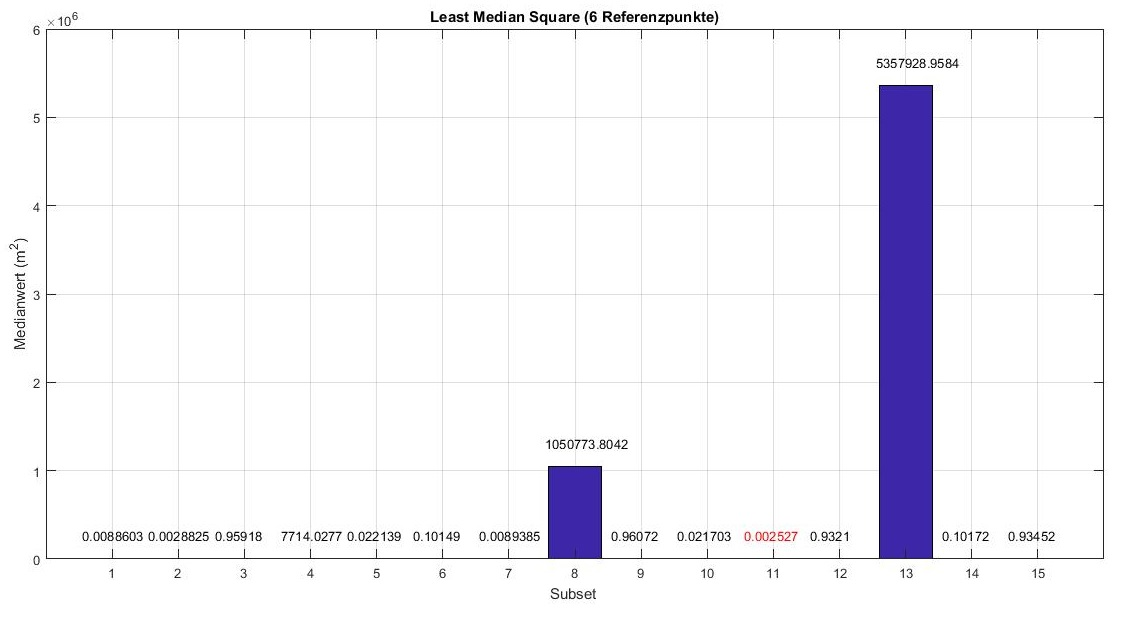
\includegraphics[scale=0.40]{img/LMS_Medianwert.jpg}\\
	\caption{Medianwert med($\vec{v}$)\textsubscript{k} bei LMS-Verfahren }
\end{figure}

\noindent
 Mit diesem Balkendiagramm ist es offensichtlich zu sehen, dass med($\vec{v}$)\textsubscript{11} den geringsten Medianwert bekommt. Die Kombination(\textit{Subset}) der optimierten Referenzpunkte sind P\textsubscript{2}, P\textsubscript{3}, P\textsubscript{4} und P\textsubscript{5}. P\textsubscript{6} mit offensichtlicher NLOS-Messung R\textsubscript{6} und P\textsubscript{1} mit kleinem Messfehler R\textsubscript{1} werden erfolgreich gefiltert. Die gesuchte Postion ist P\textsubscript{lat(11)} = (0.0399, 0.0496, -0.0322). Die gesuchte Position und optimierte Referenzpunkte werden im 3D-Umgebung angezeigt.
\begin{figure}[H]
	\centering
	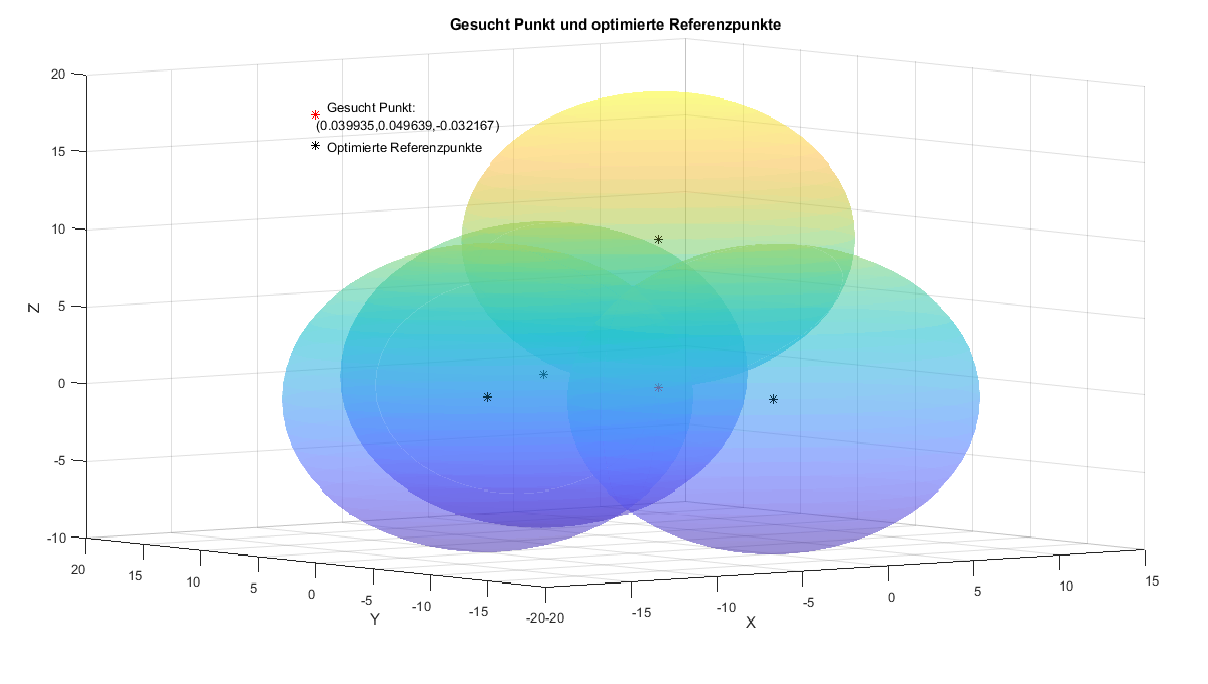
\includegraphics[scale=0.35]{img/LMS_Plat.png}\\
	\caption{Die gesucht P\textsubscript{lat(11)} und optimierte Referenzpunkte}
\end{figure}



